% adopt PLoS genetics environment settings
\documentclass[10pt,letterpaper]{article}
\usepackage[top=0.85in,left=2.75in,footskip=0.75in]{geometry}

% amsmath package, useful for mathematical formulas
\usepackage{amsmath}
%\usepackage{natbib}
% amssymb package, useful for mathematical symbols
\usepackage{amssymb}
\usepackage{booktabs}
\usepackage{xspace}
\usepackage{hyperref}
% graphicx package, useful for including eps and pdf graphics
% include graphics with the command \includegraphics
\usepackage{graphicx}


% cite package, to clean up citations in the main text. Do not remove.
\usepackage{cite}
\usepackage{caption}
\usepackage{subcaption}
\usepackage{rotating}

\usepackage{color} 

% Use doublespacing - comment out for single spacing
%\usepackage{setspace} 
%\doublespacing


% Text layout
\topmargin 0.0cm
\oddsidemargin 0.5cm
\evensidemargin 0.5cm
\textwidth 16cm 
\textheight 21cm

\setlength{\parskip}{1em}

% Bold the 'Figure #' in the caption and separate it with a period
% Captions will be left justified
\usepackage[labelfont=bf,labelsep=period,justification=raggedright]{caption}

% Use the PLoS provided bibtex style
\bibliographystyle{/Users/stephens/Dropbox/Documents/stylefiles/plos2009}

% Remove brackets from numbering in List of References
\makeatletter
\renewcommand{\@biblabel}[1]{\quad#1.}
\makeatother


% Leave date blank
\date{}

\pagestyle{myheadings}
%% ** EDIT HERE **
\usepackage{enumerate}
\usepackage{multirow} 
\usepackage{url}
\usepackage{xr} %for cross-referencing
%% ** EDIT HERE **
%% PLEASE INCLUDE ALL MACROS BELOW
\newtheorem{algorithm}{Algorithm}
\newtheorem{proposition}{Proposition}
\newtheorem{restateproposition}{Proposition}
\newtheorem{lemma}{Lemma}
\newtheorem{corollary}{Corollary}
\newtheorem{result}{Result}
\newtheorem{note}{Note}
\newtheorem{definition}{Definition}

\def\KL{\text{KL}}


% Text layout specific to Supplemental Materials
\topmargin 0.0cm
\oddsidemargin 0.5cm
\evensidemargin 0.5cm
\textwidth 16cm
\textheight 21cm

\setlength{\parskip}{1em}

\begin{document}

\paragraph*{S5 Fig.}

\begin{figure}[ht]
\centering
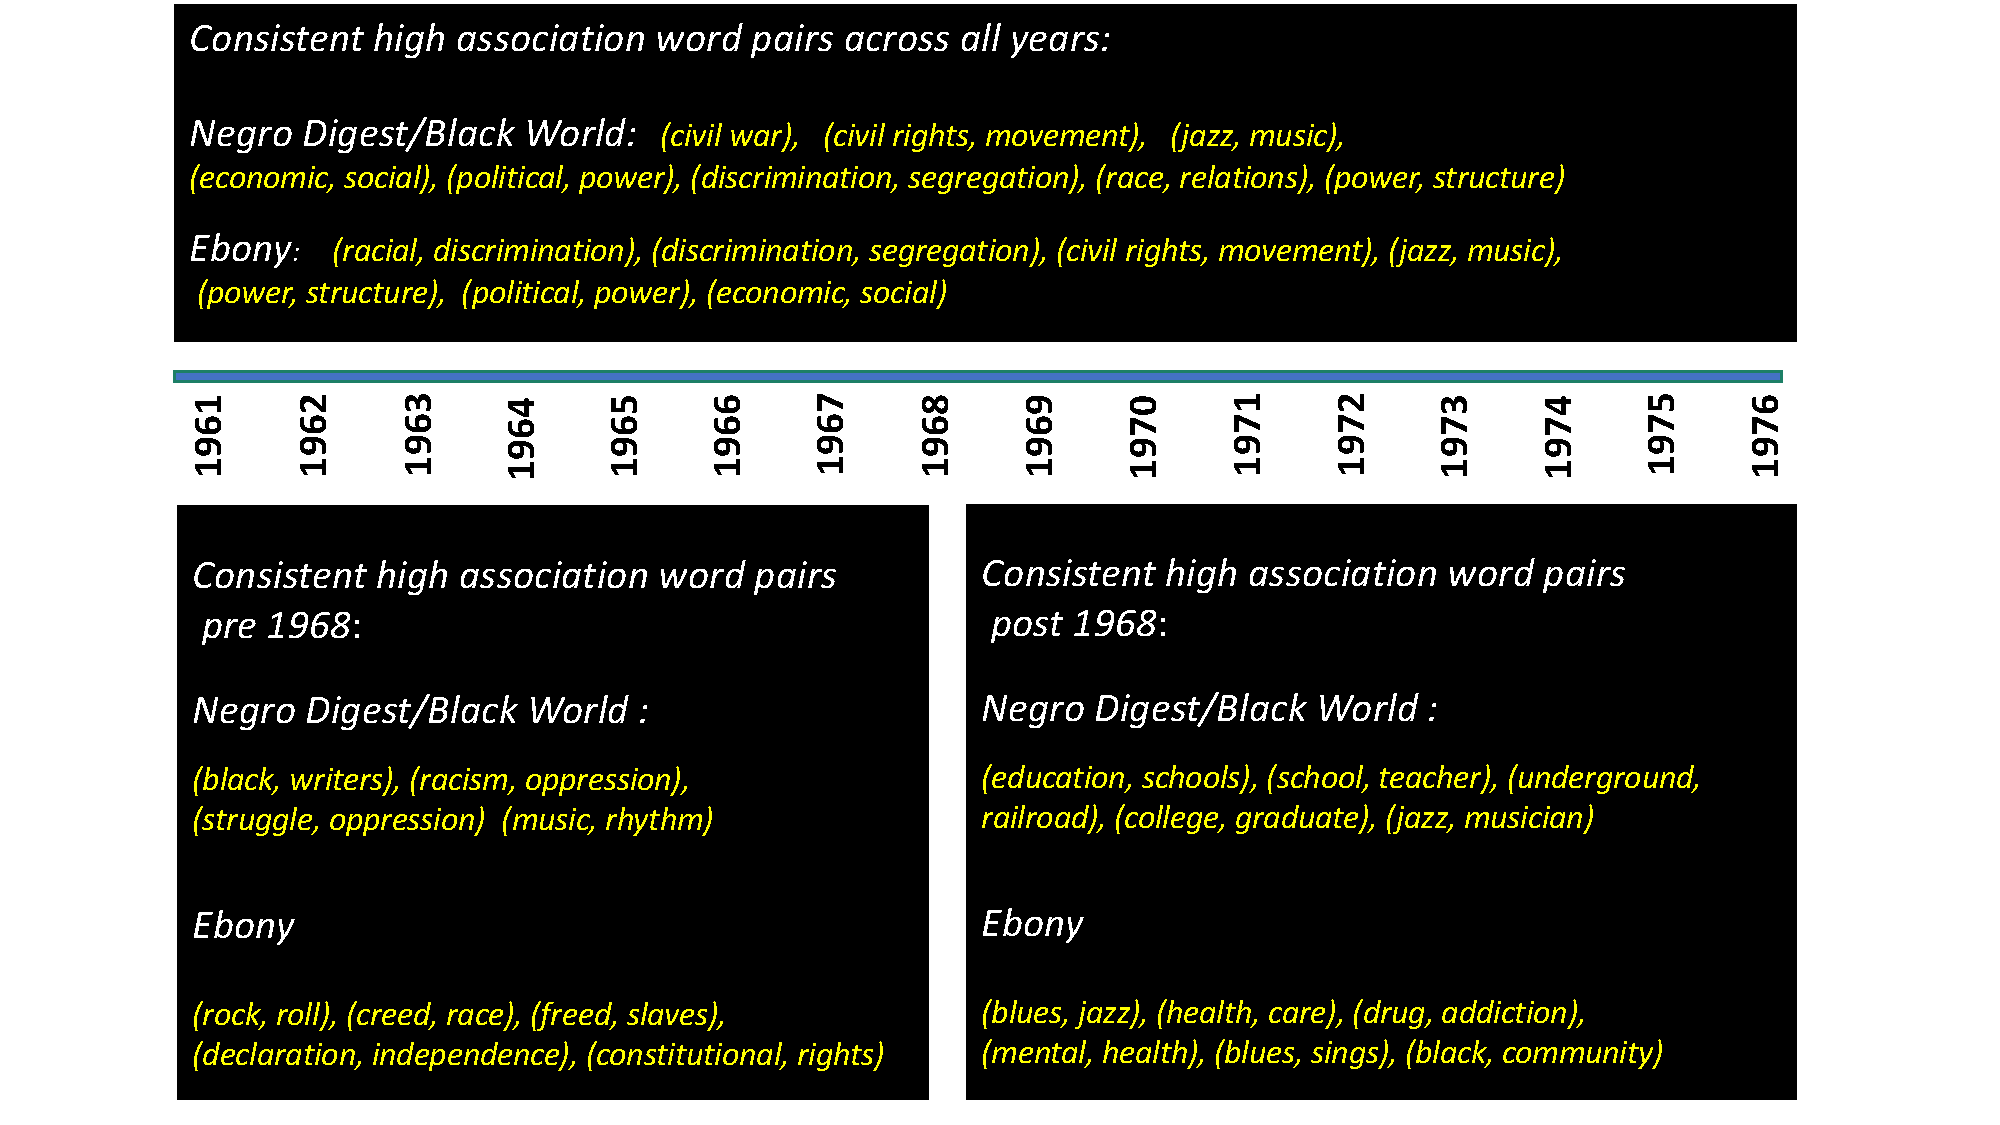
\includegraphics[height=4in, width=6in]{SuppFig5.pdf}
\end{figure}
\label{figS5}
{\bf Word pairs - presented here as \emph{(word1, word2)} - that show (A) consistently high association score throughout the period of 16 years of study (B)  much higher score pre-1968 compared to post 1968 and (C) much higher score post-1968 compared to pre-1968 . To obtain the word pairs for panels B and C, we compute the difference in median association score between post 1968 and pre 1968 texts and extract the top 10 word pairs with the highest positive and negative values of the differences. Of these 10 word pairs,  we only report the ones that are meaningful from a narrative perspective (for e.g. - devoid of names of individuals, places etc). For panel A, we report the meaningful word pairs out of the top 10 pairs with the highest median association score over the period of 16 years.
\end{document}
